\chapter{Experimentación}

En esta sección se detalla cuál fue la metodología empleada para llevar a cabo los experimentos y se detalla el algoritmo propuesto como solución. En la figura \ref{fig:metodologia} a continuación, se puede ver el panorama general de dicha metodología experimental.\\

\begin{figure}[H]
	\centering
	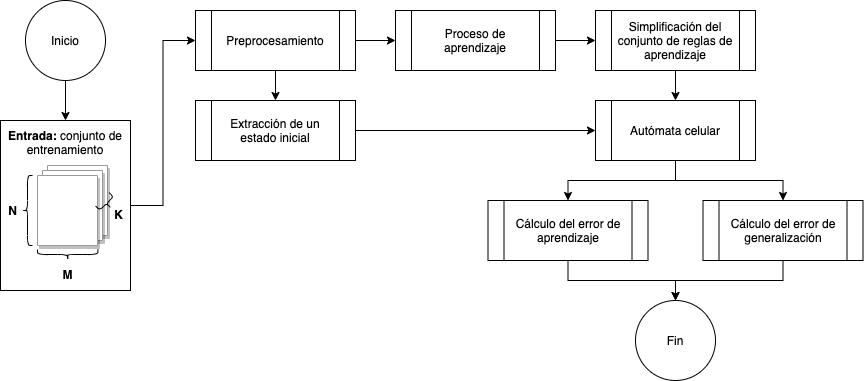
\includegraphics[width=\linewidth]{fig/metodologia}
	\caption{Diagrama general de la metodología.}
	\label{fig:metodologia}
\end{figure}

\section{Conjunto de datos}

Para realizar los experimentos, se optó por integrar un conjunto de datos que consiste en los estados de la evolución de cuatro diferentes autómatas celulares bidimensionales que fueron obtenidos de \cite{rucker_walker}.
\\

Para cada uno de los autómatas se obtuvieron 200 imágenes de 50x50 pixeles en escala RGB, que se ejemplifican en las imágenes de la Figura \ref{fig:caexamples} a continuación.

\begin{figure}[h]
	
	\begin{subfigure}{0.5\textwidth}
		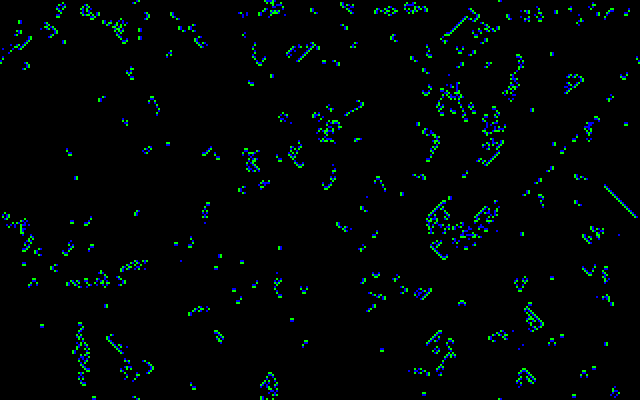
\includegraphics[width=0.9\linewidth, height=5cm]{fig/brain_1} 
		\caption{Brain estado 1}
		\label{fig:brain1}
	\end{subfigure}
	\begin{subfigure}{0.5\textwidth}
		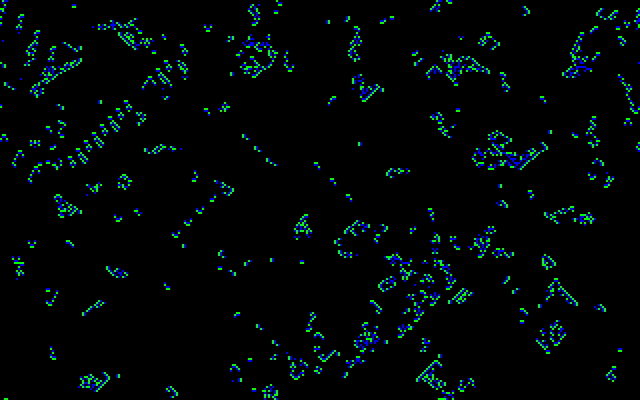
\includegraphics[width=0.9\linewidth, height=5cm]{fig/brain_200}
		\caption{Brain estado 200}
		\label{fig:brain200}
	\end{subfigure}
	\begin{subfigure}{0.5\textwidth}
		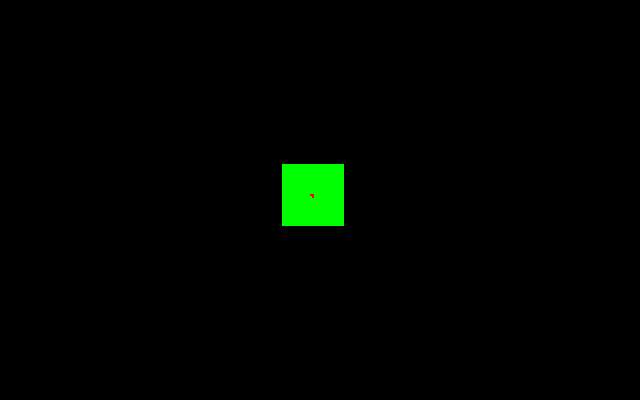
\includegraphics[width=0.9\linewidth, height=5cm]{fig/mite_1}
		\caption{Mite estado 1}
		\label{fig:mite100}
	\end{subfigure}
	\begin{subfigure}{0.5\textwidth}
		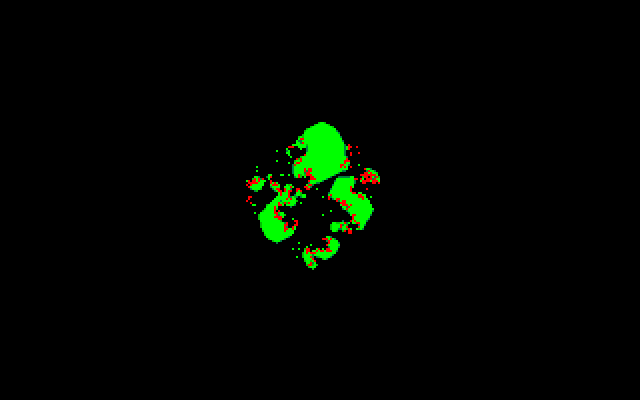
\includegraphics[width=0.9\linewidth, height=5cm]{fig/mite_200}
		\caption{Mite estado 200}
		\label{fig:mite200}
	\end{subfigure}
	
	\caption{Ejemplo del conjunto de datos}
	\label{fig:caexamples}
\end{figure}

A continuación, se mencionan los autómatas celulares en los cuales se implementaron este tipo de imágenes.

\subsection{Brain}

Es un autómata celular bidimensional, desarrollado por Brian Silverman, que modela la evolución de conjuntos de neuronas y sus interacciones. En otras palabras, el AC Brain modela cierto nivel de actividad cerebral en escenarios simples y consiste en lo siguiente:

\begin{itemize}
	\item \textbf{Vecindario:} es de tipo Moore con 8 vecinos.
	\item \textbf{Espacio de estados:} 3 estados.
	\begin{itemize}
		\item 0 que representa el estado apagado
		\item 1 que representa el estado encendido
		\item 2 que representa el estado muriendo.
	\end{itemize}
	\item \textbf{Función de evolución:} 
	\begin{itemize}
		\item 1 si se encuentra apagado y si dos o mas vecinos se encuentran encendidos.
		\item 2 si en el estado anterior estaba encendido.
		\item 0 si en el estado anterior estaba muriendo.
	\end{itemize}
\end{itemize}

\subsection{Byl}

El AC Byl \citep{BYL1989295} es un autómata celular bidimensional que fue desarrollado por Jhon Byl en 1989 con la capacidad de autoreplicarse. Este AC consiste en lo siguiente:

\begin{itemize}
	\item \textbf{Vecindario:} es de tipo Von Neumann con 5 vecinos, en el cuadro \ref{tab:bylneigh} podemos ver como se codifica el vecindario.
	\item \textbf{Espacio de estados:} consiste de 6 estados del 0 al 5.
	\item \textbf{Función de evolución:} se muestra en el cuadro \ref{tab:byltransfunction}.
\end{itemize}

\begin{table}[H]
	\begin{center}
		\renewcommand{\arraystretch}{1.3}
		\begin{tabular}{ c c c c c}
			\hline
			CTRBL $\rightarrow$ I & CTRBL $\rightarrow$ I & CTRBL $\rightarrow$ I & CTRBL $\rightarrow$ I & CTRBL $\rightarrow$ I \\ 
			\hline
			00003\quad\quad\quad 1& 10003\quad\quad\quad 3 & 20215\quad\quad\quad 5 & 31215\quad\quad\quad 1 & 40242\quad\quad\quad 4 \\  
			00012\quad\quad\quad 2& 10004\quad\quad\quad 0 & 20235\quad\quad\quad 3 & 31223\quad\quad\quad 1 & 40252\quad\quad\quad 0 \\
			00013\quad\quad\quad 1& 10033\quad\quad\quad 0 & 20252\quad\quad\quad 5 & 31233\quad\quad\quad 1 & 40325\quad\quad\quad 5  \\
			00015\quad\quad\quad 2& 10043\quad\quad\quad 1 & 2 - - - - \quad\quad 2 & 31235\quad\quad\quad 5 & 4 - - - - \quad\quad 3  \\
			00025\quad\quad\quad 5& 10321\quad\quad\quad 3 & 30001\quad\quad\quad 0 & 31432\quad\quad\quad 1 & 50022\quad\quad\quad 5 \\
			00031\quad\quad\quad 5& 11253\quad\quad\quad 1 & 30003\quad\quad\quad 0 & 31452\quad\quad\quad 5 & 50032\quad\quad\quad 5  \\
			00032\quad\quad\quad 3& 12453\quad\quad\quad 3 & 30011\quad\quad\quad 0 & 3 - - - - \quad\quad 3 & 50212\quad\quad\quad 4  \\
			00042\quad\quad\quad 2& 1 - - - - \quad\quad 4 & 30012\quad\quad\quad 1 & & 50222\quad\quad\quad 0 \\
			0 - - - - \quad\quad 0 & 20000\quad\quad\quad 0 & 30121\quad\quad\quad 1 & 40003\quad\quad\quad 0 & 50322\quad\quad\quad 0  \\
			& 20015\quad\quad\quad 5 & 30123\quad\quad\quad 1 & 40043\quad\quad\quad 0 & 5 - - - - \quad\quad 2  \\
			10000\quad\quad\quad 0& 20022\quad\quad\quad 0 & 31122\quad\quad\quad 1 & 40212\quad\quad\quad 0 & \\
			10001\quad\quad\quad 0& 20202\quad\quad\quad 0 & 31123\quad\quad\quad 1 & 40232\quad\quad\quad 0 &
		\end{tabular}
		\caption{\label{tab:byltransfunction} Función de evolución de Byl CA \citep{BYL1989295}.}
	\end{center}
\end{table}

\begin{table}[H]
	\begin{center}
		\begin{tabular}{ c c c}
			&T&\\
			L&C&R $\rightarrow$ I\\
			&B&\\
		\end{tabular}
	\end{center}
	\caption{\label{tab:bylneigh} Codificación del vecindario.}
\end{table}

\subsection{Evoloops}
El AC Evoloops \citep{Sayama1998ConstructingES} es un autómata celular bidimensional, desarrollado por Hiroki Sayama para autoreplicarse, consiste en lo siguiente:
\begin{itemize}
	\item \textbf{Vecindario:} es de tipo Von Neumann con 5 vecinos, en el cuadro \ref{tab:bylneigh} podemos ver como se codifica el vecindario.
	\item \textbf{Espacio de estados:} consiste de 8 estados del 0 al 7.
	\item \textbf{Función de evolución:} se muestra en el cuadro \ref{tab:evoloopstransfunction}.
\end{itemize}

\begin{table}[H]
	\begin{center}
		\renewcommand{\arraystretch}{1.2}
		\resizebox{\textwidth}{!}{%
			\begin{tabular}{ c c c c c c}
				\hline
				CTRBL $\rightarrow$ I & CTRBL $\rightarrow$ I & CTRBL $\rightarrow$ I & CTRBL $\rightarrow$ I & CTRBL $\rightarrow$ I & CTRBL $\rightarrow$ I \\ 
				\hline
				00001\quad\quad\quad2& 10202\quad\quad\quad1& 11272\quad\quad\quad7& 20172\quad\quad\quad2& 21322\quad\quad\quad2& 40125\quad\quad\quad0\\
				00004\quad\quad\quad3& 10211\quad\quad\quad1& 11273\quad\quad\quad5& 20202\quad\quad\quad2& 21422\quad\quad\quad2& 40162\quad\quad\quad0\\
				00012\quad\quad\quad2& 10212\quad\quad\quad1& 11322\quad\quad\quad1& 20203\quad\quad\quad2& 21622\quad\quad\quad2& 40212\quad\quad\quad0\\
				00015\quad\quad\quad2& 10213\quad\quad\quad1& 11332\quad\quad\quad1& 20205\quad\quad\quad2& 21722\quad\quad\quad2& 40215\quad\quad\quad0\\
				00021\quad\quad\quad2& 10221\quad\quad\quad1& 11542\quad\quad\quad4& 20206\quad\quad\quad5& 22224\quad\quad\quad2& 40222\quad\quad\quad1\\
				00024\quad\quad\quad2& 10224\quad\quad\quad4& 11572\quad\quad\quad7& 20207\quad\quad\quad3& 22227\quad\quad\quad2& 40232\quad\quad\quad1\\
				00042\quad\quad\quad2& 10227\quad\quad\quad7& 11624\quad\quad\quad4& 20212\quad\quad\quad2& 22234\quad\quad\quad2& 40262\quad\quad\quad6\\
				00045\quad\quad\quad2& 10232\quad\quad\quad4& 11627\quad\quad\quad7& 20215\quad\quad\quad2& 22237\quad\quad\quad2& 40312\quad\quad\quad0\\
				00075\quad\quad\quad2& 10241\quad\quad\quad4& 12224\quad\quad\quad4& 20221\quad\quad\quad2& 22243\quad\quad\quad2& 40322\quad\quad\quad1\\
				00102\quad\quad\quad2& 10242\quad\quad\quad4& 12227\quad\quad\quad7& 20222\quad\quad\quad2& 22244\quad\quad\quad2& 50002\quad\quad\quad5\\
				00214\quad\quad\quad1& 10243\quad\quad\quad4& 12243\quad\quad\quad4& 20223\quad\quad\quad2& 22273\quad\quad\quad2& 50012\quad\quad\quad5\\
				00217\quad\quad\quad1& 10251\quad\quad\quad1& 12273\quad\quad\quad7& 20232\quad\quad\quad3& 22277\quad\quad\quad2& 50021\quad\quad\quad5\\
				00232\quad\quad\quad2& 10252\quad\quad\quad7& 12324\quad\quad\quad4& 20242\quad\quad\quad2& 22324\quad\quad\quad3& 50023\quad\quad\quad2\\
				01122\quad\quad\quad1& 10254\quad\quad\quad3& 12327\quad\quad\quad7& 20245\quad\quad\quad2& 22327\quad\quad\quad3& 50024\quad\quad\quad5\\
				01212\quad\quad\quad1& 10257\quad\quad\quad7& 12426\quad\quad\quad6& 20252\quad\quad\quad5& 30001\quad\quad\quad3& 50027\quad\quad\quad5\\
				01232\quad\quad\quad1& 10271\quad\quad\quad7& 12433\quad\quad\quad3& 20262\quad\quad\quad0& 30002\quad\quad\quad2& 50042\quad\quad\quad5\\
				01242\quad\quad\quad1& 10272\quad\quad\quad7& 12627\quad\quad\quad6& 20265\quad\quad\quad0& 30003\quad\quad\quad2& 50072\quad\quad\quad5\\
				01245\quad\quad\quad1& 10273\quad\quad\quad5& 20001\quad\quad\quad2& 20272\quad\quad\quad2& 30004\quad\quad\quad3& 50202\quad\quad\quad2\\
				01252\quad\quad\quad6& 10512\quad\quad\quad1& 20002\quad\quad\quad2& 20275\quad\quad\quad2& 30007\quad\quad\quad4& 50205\quad\quad\quad2\\
				01262\quad\quad\quad6& 10542\quad\quad\quad4& 20004\quad\quad\quad2& 20312\quad\quad\quad2& 30012\quad\quad\quad3& 50212\quad\quad\quad5\\
				
		\end{tabular}}
	\end{center}
\end{table}
\begin{table}[H]
	\begin{center}
		\renewcommand{\arraystretch}{1.2}
		\resizebox{\textwidth}{!}{%
			\begin{tabular}{ c c c c c c}
				01272\quad\quad\quad1& 10572\quad\quad\quad7& 20005\quad\quad\quad2& 20322\quad\quad\quad2& 30032\quad\quad\quad2& 50215\quad\quad\quad2\\
				01275\quad\quad\quad1& 10621\quad\quad\quad1& 20006\quad\quad\quad0& 20342\quad\quad\quad2& 30042\quad\quad\quad1& 50242\quad\quad\quad5\\
				01342\quad\quad\quad1& 10624\quad\quad\quad4& 20007\quad\quad\quad1& 20345\quad\quad\quad2& 30102\quad\quad\quad1& 50272\quad\quad\quad5\\
				01372\quad\quad\quad1& 10627\quad\quad\quad7& 20012\quad\quad\quad2& 20372\quad\quad\quad2& 30125\quad\quad\quad0& 50312\quad\quad\quad0\\
				01422\quad\quad\quad1& 11112\quad\quad\quad1& 20015\quad\quad\quad2& 20412\quad\quad\quad2& 30212\quad\quad\quad3& 60202\quad\quad\quad2\\
				01425\quad\quad\quad1& 11122\quad\quad\quad1& 20021\quad\quad\quad2& 20422\quad\quad\quad2& 30242\quad\quad\quad3& 60212\quad\quad\quad2\\
				01432\quad\quad\quad1& 11124\quad\quad\quad4& 20022\quad\quad\quad2& 20442\quad\quad\quad2& 30252\quad\quad\quad1& 60222\quad\quad\quad0\\
				01435\quad\quad\quad1& 11125\quad\quad\quad1& 20023\quad\quad\quad2& 20512\quad\quad\quad2& 30272\quad\quad\quad3& 60242\quad\quad\quad2\\
				01442\quad\quad\quad1& 11127\quad\quad\quad7& 20024\quad\quad\quad2& 20542\quad\quad\quad5& 30332\quad\quad\quad1& 60272\quad\quad\quad2\\
				01462\quad\quad\quad1& 11162\quad\quad\quad1& 20026\quad\quad\quad0& 20572\quad\quad\quad5& 31212\quad\quad\quad3& 61222\quad\quad\quad0\\
				01722\quad\quad\quad1& 11212\quad\quad\quad1& 20027\quad\quad\quad2& 20612\quad\quad\quad5& 31242\quad\quad\quad3& 62224\quad\quad\quad0\\
				01725\quad\quad\quad1& 11213\quad\quad\quad1& 20032\quad\quad\quad4& 20621\quad\quad\quad2& 31252\quad\quad\quad1& 62227\quad\quad\quad0\\
				01756\quad\quad\quad1& 11215\quad\quad\quad1& 20042\quad\quad\quad3& 20642\quad\quad\quad5& 31272\quad\quad\quad3& 70102\quad\quad\quad0\\
				01762\quad\quad\quad1& 11222\quad\quad\quad1& 20045\quad\quad\quad2& 20672\quad\quad\quad5& 32424\quad\quad\quad3& 70112\quad\quad\quad0\\
				01772\quad\quad\quad1& 11224\quad\quad\quad4& 20054\quad\quad\quad5& 20712\quad\quad\quad2& 32425\quad\quad\quad1& 70122\quad\quad\quad0\\
				10001\quad\quad\quad1& 11227\quad\quad\quad7& 20057\quad\quad\quad5& 20722\quad\quad\quad2& 32427\quad\quad\quad3& 70125\quad\quad\quad0\\
				10012\quad\quad\quad1& 11232\quad\quad\quad1& 20062\quad\quad\quad0& 20772\quad\quad\quad2& 32527\quad\quad\quad1& 70162\quad\quad\quad0\\
				10021\quad\quad\quad1& 11242\quad\quad\quad4& 20072\quad\quad\quad2& 21122\quad\quad\quad2& 32727\quad\quad\quad3& 70212\quad\quad\quad0\\
				10024\quad\quad\quad4& 11243\quad\quad\quad4& 20075\quad\quad\quad2& 21222\quad\quad\quad2& 40000\quad\quad\quad1& 70215\quad\quad\quad0\\
				10027\quad\quad\quad7& 11252\quad\quad\quad7& 20102\quad\quad\quad2& 21223\quad\quad\quad2& 40002\quad\quad\quad1& 70222\quad\quad\quad1\\
				10121\quad\quad\quad1& 11254\quad\quad\quad3& 20112\quad\quad\quad2& 21224\quad\quad\quad2& 40102\quad\quad\quad0& 70232\quad\quad\quad0\\
				10124\quad\quad\quad4& 11257\quad\quad\quad7& 20122\quad\quad\quad2& 21227\quad\quad\quad2& 40112\quad\quad\quad0& 70262\quad\quad\quad6\\
				10127\quad\quad\quad7& 11262\quad\quad\quad6& 20142\quad\quad\quad2& 21232\quad\quad\quad3& 40122\quad\quad\quad0& 70312\quad\quad\quad0
		\end{tabular}}
		\caption{\label{tab:evoloopstransfunction} Función de evolución de Evoloops CA \citep{Sayama1998ConstructingES}.}
	\end{center}
\end{table}

\subsection{Mite}

El AC Mite es un autómata celular bidimensional, desarrollado por Dan Drake en 1990, que modela el sistema presa-depredador y consiste en lo siguiente:
\begin{itemize}
	\item \textbf{Vecindario:} es de tipo Moore con 8 vecinos.
	\item \textbf{Espacio de estados:} consiste de 3 estados del 0 al 2.
	\item \textbf{Función de evolución:} 
	\begin{itemize}
		\item mover la posición del predador de manera aleatoria dentro de su vecindario local.
		\item si no hay presa en su posición el predador muere.
		\item si hay suficientes presas en su posición se incrementa el número de predadores.
		\item si hay dos presas juntas se incrementa el número de presas.
	\end{itemize}
\end{itemize}

\section{Preprocesamiento}
Una vez adquiridas las secuencias de imágenes de cada autómata celular, se continúa con los procesos de discretización y binarización que se explican en las subsecciones siguientes.

En términos generales, la discretización consta en pasar las imágenes de los canales RGB a valores discretos, mientras que el proceso de binarización solo se realiza para los datos que se van a ingresar al algoritmo RA1. De cualquier manera, se mencionan a continuación algunas características específicas de cada proceso.

\subsection{Discretización}

La implementación de este procedimiento se realizó en el lenguaje Python y se ejemplifica con el siguiente pseudocódigo.

\begin{algorithm}[H] 
	\SetKwInOut{Input}{entrada}
	\SetKwInOut{Output}{salida}
	\Input{La ruta de la carpeta donde se encuentran las imágenes}
	\Output{Un archivo con formato .pkl que contiene las imágenes procesadas.}
	\SetAlgoLined
	diccionario = \{\} ; contador = 0; imágenes=[ ] \tcc*{inicializaciones}
	\ForEach{$Imagen$ en $carpeta$}{
		\textbf{Paso 1:}$Imagen'=$   Transformar imagen a escala de grises\;
		\tcc{Se considera a la imagen como una matriz de pixeles}
		nuevaImagen = [ ]\;
		\ForEach{fila en Imagen}{
			\tcc{una fila es un arreglo de pixeles}
			nuevaFila = [ ] \;
			\ForEach{pixel en fila}{ 
				\tcc{un pixel corresponde a un valor entre 0 y 255 despues de la transformación}
				\If{pixel no esta en diccionario}{
					\textbf{Paso 2:} diccionarion[pixel] = contador\;
					\textbf{Paso 3:} contador = contador + 1\;
				}
				\textbf{Paso 4:} nuevaFila.agregar(diccionario[pixel])\;
			}
			\textbf{Paso 5:} nuevaImagen.agregar(nuevaFila)\;
		}
		\textbf{Paso 6:} imagenes.agregar(nuevaImagen)\;
	}
	\textbf{Paso 7:} Guardar imágenes en formato .pkl\;
	\caption{Pseudocódigo para la discretización de las imágenes.}
\end{algorithm}

\subsection{Binarización}

Este proceso se realiza solamente para los datos que ingresarán al algoritmo RA1 debido a que este algoritmo solo es capaz de aprender de datos categóricos. El siguiente pseudocódigo ejemplifica este proceso.

\begin{algorithm}[H] 
	\SetKwInOut{Input}{entrada}
	\SetKwInOut{Output}{salida}
	\Input{MEstado: matriz de estado}
	\Output{El estado binarizado}
	\SetAlgoLined
	nuevoEstado = []\;
	\ForEach{fila en MEstado}{
		\textbf{nuevaFila} = []\;
		\ForEach{celda en fila}{
			\textbf{Paso 1:} Encontrar el dominio de la celda\;
			\textbf{Paso 2:} dominio = ordenarAscendente (dominio)\;
			\ForEach{valor en dominio}{
				\eIf{celda < valor}{
					\textbf{Paso 3a:} nuevaFila.agregar(1)\;
				}{
					\textbf{Paso 3b:} nuevaFila.agregar(0)\;
				}
			}
			
		}
		\textbf{Paso 4:} nuevoEstado.agregar(nuevaFila)\;
	}
	
	\caption{Pseudocódigo para la binarización de las imágenes.}
\end{algorithm}

\section{Algoritmos de aprendizaje}
Los algoritmos de aprendizaje utilizados en este trabajo de investigación son los siguientes:
\begin{itemize}
	\item RA1
	\item GA-Nuggets
	\item LRDEA el algoritmo diseñado en este trabajo.
\end{itemize}

Cabe mencionar que, debido a que no se encontraron las implementaciones de los algoritmos RA1 y GA-Nuggets, fue necesario realizarlas en el lenguaje de programación Python.

\section{Simplificación de reglas}

El proceso de simplificación de reglas se divide en dos partes:
\begin{enumerate}
	\item remover redundancia en las cláusulas.
	\item emplear el algoritmo Quine–McCluskey para minimizar las cláusulas.
\end{enumerate}

El primer método de simplificación sirve para eliminar términos que no aportan aportan nueva información, esto es por que otros términos contienen a estos. En el siguiente ejemplo podemos ver como es este proceso.

\begin{figure}[H]
	\centering
	\includegraphics[width=\linewidth]{fig/clausulas}
	\caption{Ejemplo del proceso de simplificación 1.}
	\label{fig:simp1}
\end{figure}

En el diagrama de la figura \ref{fig:simp1} vemos cómo, en la cláusula \emph{a}, los términos 1 y 2 pueden ser reducidos a los términos 4 y 5 de la cláusula \emph{b}, respectivamente. Asimismo, podemos ver cómo el término 3 de \emph{a} no se puede reducir, por lo que pasa a \emph{b} directamente.
\\

Para la simplificación 2 de las reglas se utiliza el algoritmo desarrollado por Willard V.Quine 1955 y extendido Edward J. McCluskey en 1956. Este mecanismo solo se emplea para la simplificación de las reglas generadas por el algoritmo RA1.

\section{Evaluación}

En el proceso de evaluación se emplea la validación \emph{camina hacia adelante} o \emph{Walk-Forward}, que se ejemplifica en el Algoritmo \ref{walkforward}.

\begin{algorithm}[H] 
	\SetAlgoLined
	\tcc{el rango va del 80\% del total de datos al 100\%}
	\ForEach{i en rango(160,200) }{
		\tcc{tomamos un subconjunto del conjunto de datos}
		\textbf{Paso 1:} entrenamiento = datos[0:(i-1)]\; 
		\tcc{tomamos un elemento adicional del conjunto de datos}
		\textbf{Paso 2:} testing = datos[i] \;
		\tcc{aprendemos del conjunto de entrenamiento}
		\textbf{Paso 3:} aprender(entrenamiento)\;
		\textbf{Paso 4:} vExactitud = exactitud(entrenamiento[i-1])\;
		\textbf{Paso 5:} tExactitud = exactitud(testing)\;
	}
	\caption{Pseudocódigo de validación de caminata hacia adelante (Walk-Forward). } \label{walkforward}
\end{algorithm}

\vspace{0.5cm}
La toma de los subconjuntos de datos se representa en la figura \ref{fig:walkforward}, donde podemos observar la dinámica de ''caminar'' hacia adelante.

\begin{figure}[H]
	\centering
	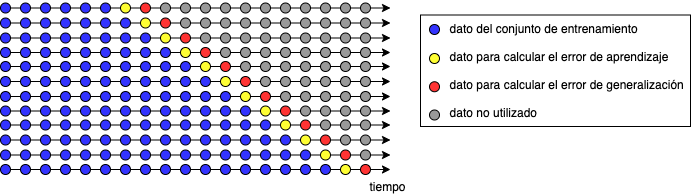
\includegraphics[width=\linewidth]{fig/walkforward}
	\caption{Diagrama de evaluación camina hacia adelante (Walk-Forward) obtenida de \cite{hyndman2018forecasting}.}
	\label{fig:walkforward}
\end{figure}

Por último, como métrica de desempeño del autómata propuesto, se emplea la \emph{exactitud} (ecuación \ref{eq:exactitud}) para calcular el error de aprendizaje y el error de generalización.

\begin{equation} \label{eq:exactitud}
exactitud = \frac{VP + VN}{VP+FP+VN+FN} 
\end{equation}

donde:
\begin{itemize}
	\item $VP:$ verdaderos positivos.
	\item $VN:$ verdaderos negativos.
	\item $FP:$ falsos positivos.
	\item $FN:$ falsos negativos. 
\end{itemize}

Esta técnica de evaluación, es comúnmente utilizada para la evaluación de series de tiempo, debido a permite evaluar cómo se comportaría el sistema de forma general en ventanas de tiempo. Adicionalmente, en específico para este trabajo, esta técnica evalúa cómo se comportarían las reglas aprendidas por el algoritmo LRDEA, una vez que se ingresen al autómata celular y se realice la simulación del fenómeno por un periodo de tiempo.


\nomenclature{VP}{Verdaderos Positivos}
\nomenclature{VN}{Verdaderos Negativos}
\nomenclature{FP}{Falsos Positivos}
\nomenclature{FN}{Falsos Negativos}
\nomenclature{LRDEA}{Local Rule Discovery Evolutive Algorithm}
\nomenclature{RGB}{Red Green Blue}